\documentclass[12pt]{article}
\usepackage{geometry}                % See geometry.pdf to learn the layout options. There are lots.
\geometry{letterpaper}                   % ... or a4paper or a5paper or ... 
%\geometry{landscape}                % Activate for for rotated page geometry
\usepackage[parfill]{parskip}    % Activate to begin paragraphs with an empty line rather than an indent
\usepackage{daves,fancyhdr,natbib,graphicx,dcolumn,amsmath,lastpage,url}
\usepackage{amsmath,amssymb,epstopdf,longtable}
\DeclareGraphicsRule{.tif}{png}{.png}{`convert #1 `dirname #1`/`basename #1 .tif`.png}
\pagestyle{fancy}
\lhead{CE 3354 -- Engineering Hydrology}
\rhead{FALL 2022}
\lfoot{ES-16}
\cfoot{}
\rfoot{Page \thepage\ of \pageref{LastPage}}
\renewcommand\headrulewidth{0pt}



\begin{document}
\begin{center}
{\textbf{{ CE 3354 Engineering Hydrology} \\ {Exercise Set 16}}}
\end{center}

\section*{\small{Exercises}}

\begin{enumerate}
\item Figure \ref{fig:porosity.pdf} depicts a cubic meter of material that when saturated contains 0.26 cubic meters of liquid.
\begin{figure}[h!] %  figure placement: here, top, bottom, or page
   \centering
   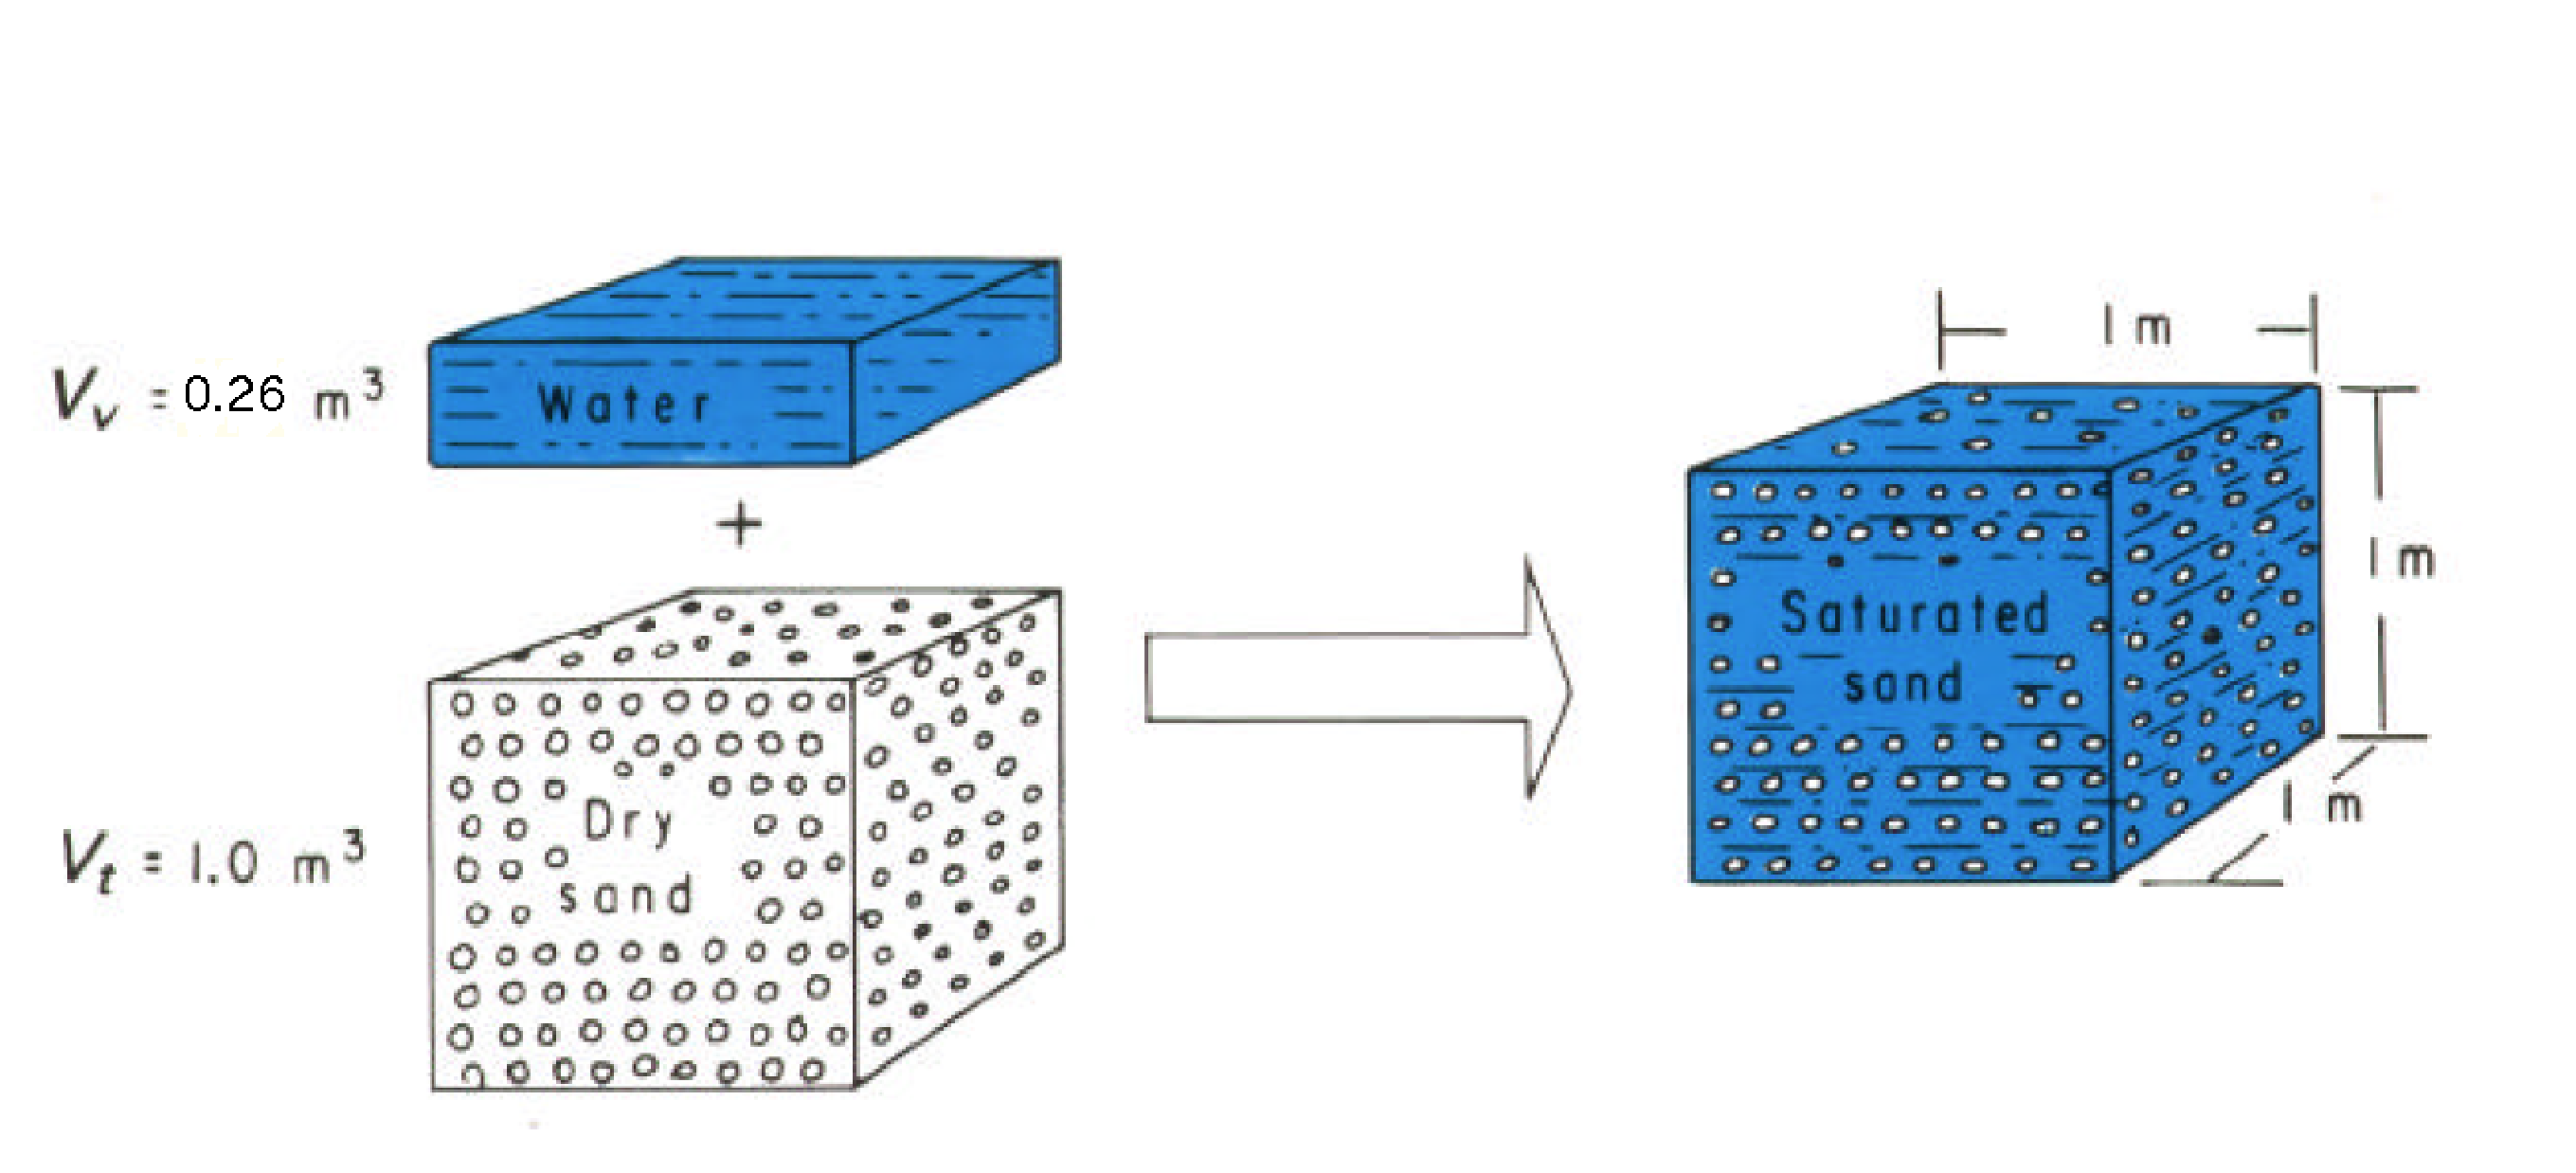
\includegraphics[width=3in]{porosity.pdf} 
   \caption{Cubic meter of saturated geologic material}
   \label{fig:porosity.pdf}
\end{figure}

\begin{enumerate}
\item What is the volume of voids in the material?
\item Write the equation that relates void volume ($V_v$), sample volume($V_b$), and porosity ($n$).
\item If the density of the liquid is 9800 N/$m^3$, what would be the weight change of a saturated sample is completely dried (all liquid removed)?  Show your arithmetic.
\end{enumerate}

\clearpage

%%%%%%%%%%%%%%%%%%%%%%%%%%%%%%%%%%%%%%%%%%%%%%%%%%%%%%%%%%%%%%%%%%%%%%
\item Water flows through the aquifer system shown in Figure \ref{fig:aquifer-77.pdf}.  The heads in the two monitoring wells are 77.0 m and 71.0 m. 
\begin{figure}[h!] %  figure placement: here, top, bottom, or page
   \centering
   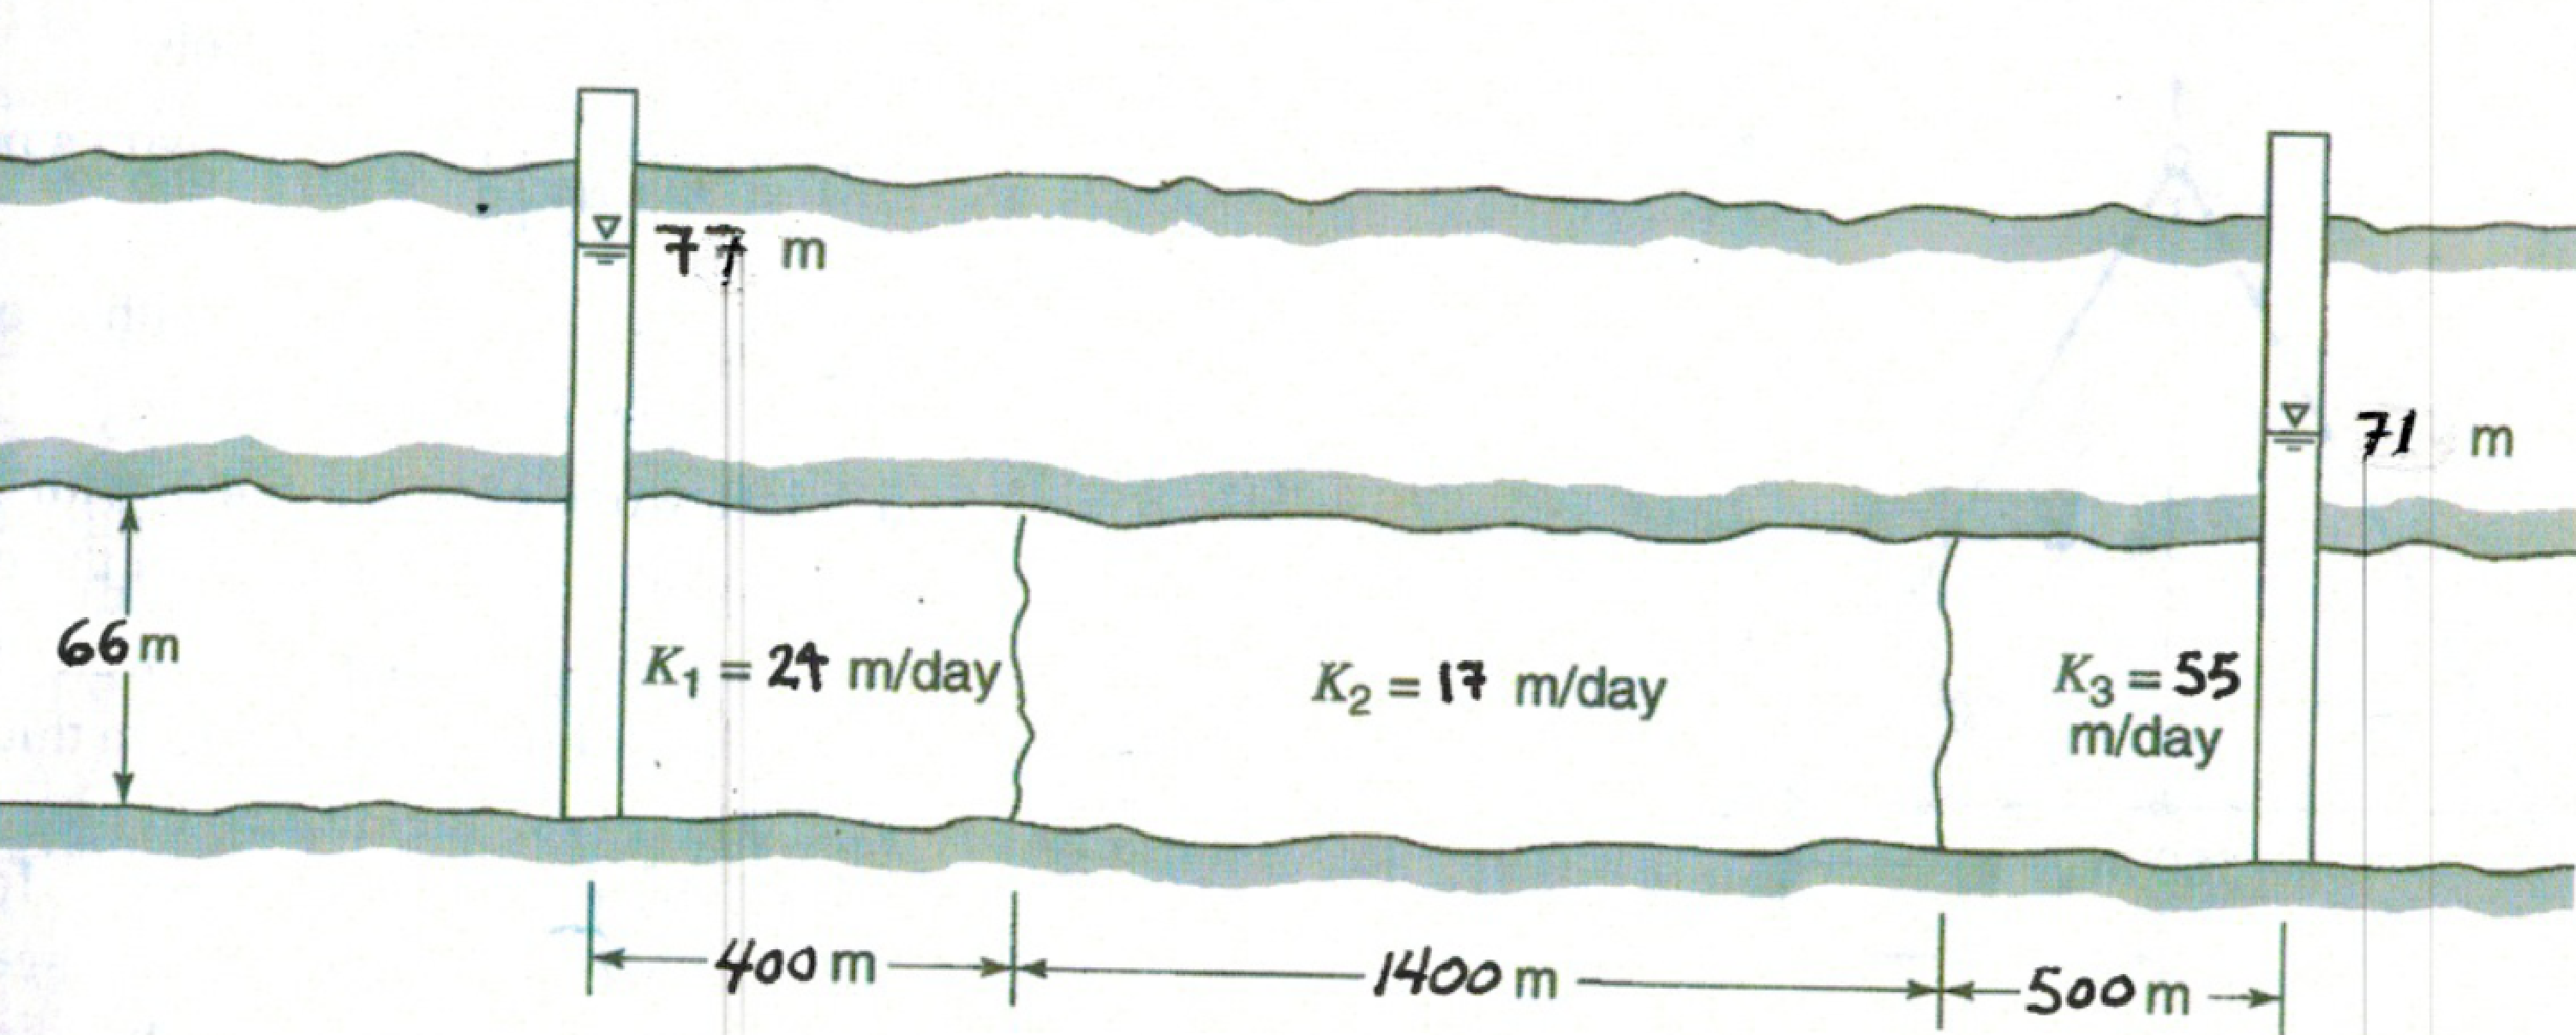
\includegraphics[width=4in]{aquifer-77.pdf} 
   \caption{Confined aquifer system with three formations in series}
   \label{fig:aquifer-77.pdf}
\end{figure}
\begin{enumerate}
\item Write the equation for flow rate through a 1-meter wide (into the figure) portion of aquifer.
\item Using the equation, estimate flow rate through a 1-meter wide (into the figure) portion of aquifer.
\end{enumerate}

\clearpage
%%%%%%%%%%%%%%%%%%%%%%%%%%%%%%%%%%%%%%%%%%%%%%%%%%%%%%%%%%%%%%%%%%%%%%%%%%%%%%%%%%

\item Three wells monitor water levels in a confined aquifer.  Well MW-A is located 3000 feet south of Well MW-B.   Well MW-C is located 2000 feet due west of Well MW-B.
The top of casing (TOC) elevations for the three wells are 480 feet, 610 feet, and 545 feet.   The depth to water (DTW) in the three wells are 40 feet, 140 feet, and 85 feet.   Table \ref{tab:piezometer-data} is a listing of these values.

% Requires the booktabs if the memoir class is not being used
\begin{table}[htbp]
   \centering
   \caption{Casing elevations and depth to water in three monitoring wells.}
   \begin{tabular}{p{1in}p{1in}p{1in}p{1in}} % Column formatting, @{} suppresses leading/trailing space
Well & TOC (feet) & DTW (feet) & Head (feet) \\
\hline
\hline
MW-A & 480 & 40 & ~ \\
~ & ~ & ~ & ~ \\
MW-B & 610 & 140 & ~ \\
~ & ~ & ~ & ~ \\
MW-C & 545 & 85 & ~  \\
\hline
\end{tabular}
\label{tab:piezometer-data}
\end{table}

Figure \ref{fig:side-view-well.pdf} is a sketch that shows the relationship between the top of casing elevation, depth to water, and head in the confined aquifer.

\begin{figure}[h!] %  figure placement: here, top, bottom, or page
   \centering
   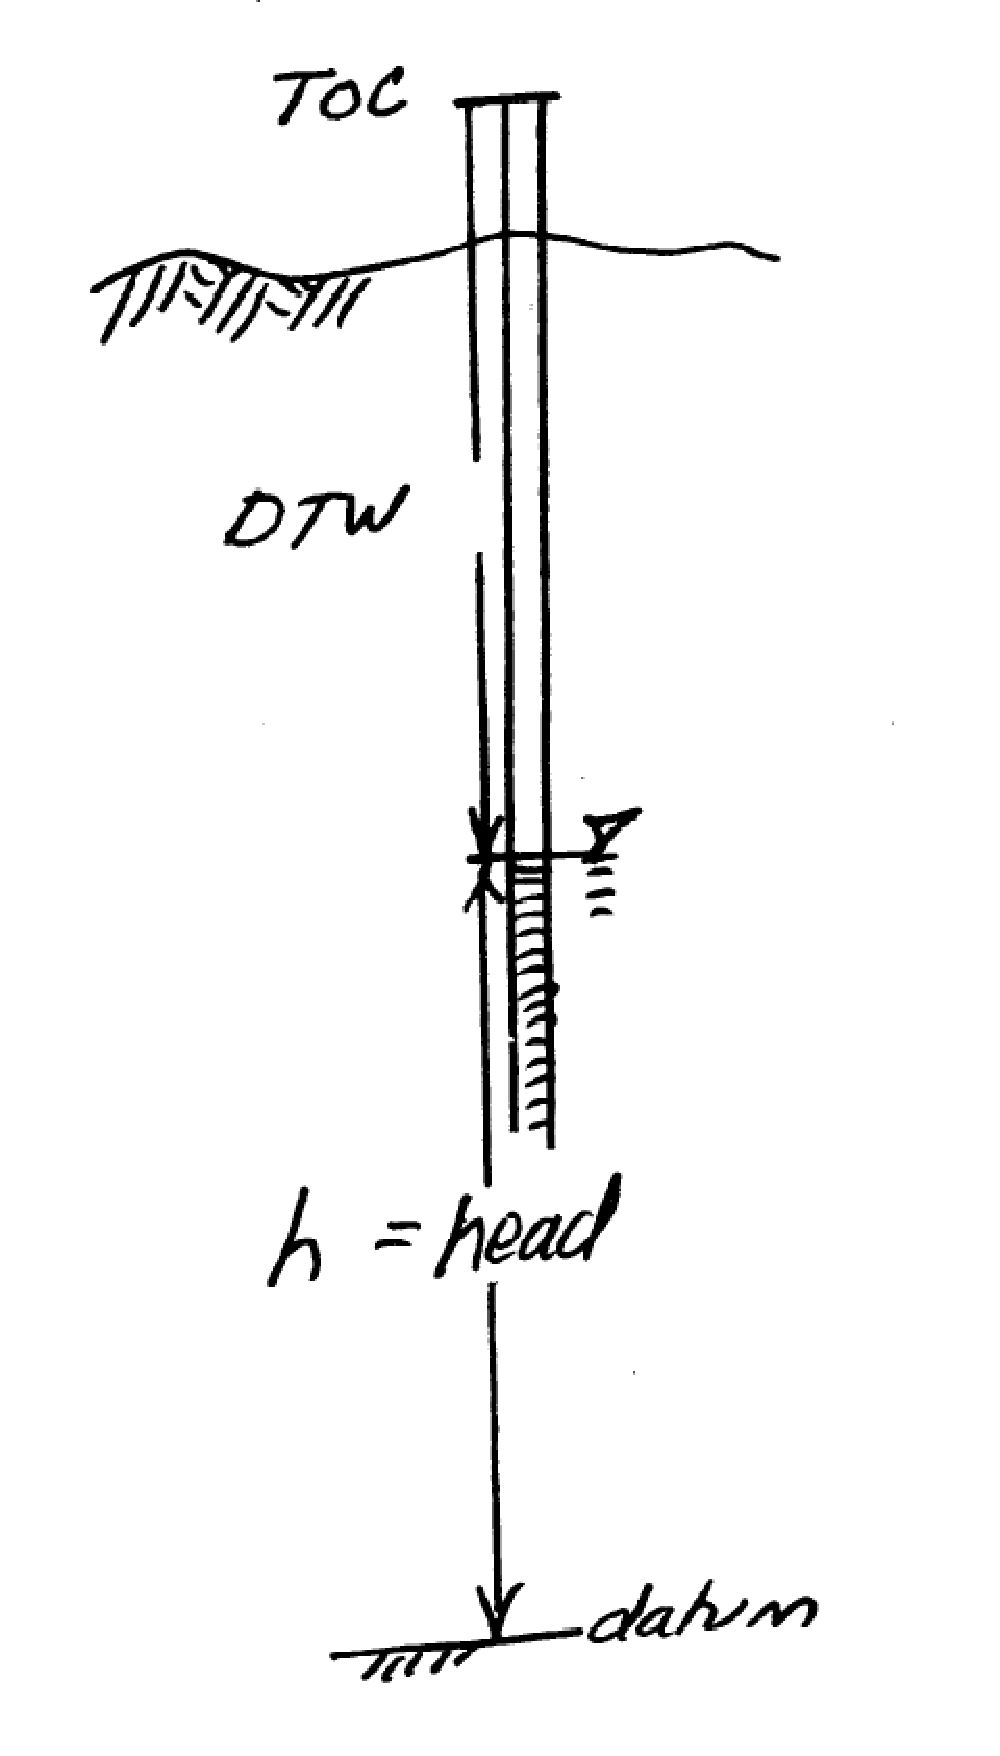
\includegraphics[height=2.5in]{side-view-well.pdf} 
   \caption{Sketch showing the relationship of top of casing (TOC) and depth to water (DTW)}
   \label{fig:side-view-well.pdf}
\end{figure}

\begin{enumerate}
\item Using Figure \ref{fig:side-view-well.pdf} as a guide, write the formula to convert the depth-to-water (DTW) measurements and top-of-casing (TOC) values into head.
\item Using Figure \ref{fig:side-view-well.pdf} as a guide, compute the head in MW-A.   Show your arithmetic.
\item Using Figure \ref{fig:side-view-well.pdf} as a guide, compute the head in MW-B.   Show your arithmetic.
\item Using Figure \ref{fig:side-view-well.pdf} as a guide, compute the head in MW-C.   Show your arithmetic.
\item Complete Table \ref{tab:piezometer-data} by entering your values computed above into the table.
%%%%%%%%%%%%%%%%%%%%%%%%%%%%%%%%%%%%%%%%%%%%%

\item A sketch of the orientation of the three wells is shown on Figure \ref{fig:grid-paper.pdf} (Next Page).   Write the value of head you computed next to each well on the sketch.
\item Determine the direction of flow using three-well triangulation.  Show your arithmetic.
\item Draw a flowline that passes through MW-B
\item Draw and label the equipotential line that passes through well MW-B.
\item Draw and label the equipotential line that passes through well MW-C.
\item Determine the distance along the flowline between the two equipotential lines.
\item Estimate the magnitude of the hydraulic gradient.

\begin{figure}[h!] %  figure placement: here, top, bottom, or page
   \centering
   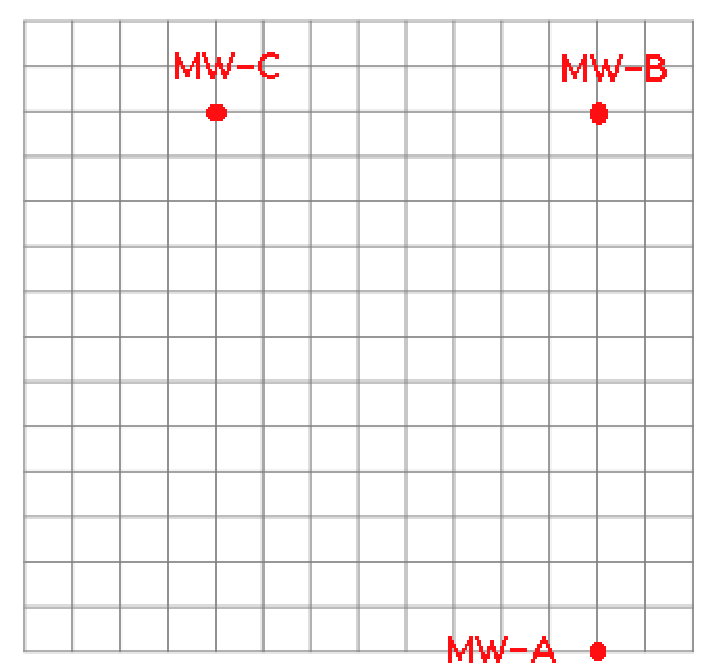
\includegraphics[width=6in]{grid-paper.pdf} 
   \caption{Three-wells monitoring a confined aquifer.}
   \label{fig:grid-paper.pdf}
\end{figure}
\clearpage


\end{enumerate}
%%%%%%%%%%%%%%%%%%%%%%%%%%%%%%%%%%%%%%%%%%%%%%%%%%%%%%%%
\clearpage
\item A well in the center of a circular island (an unconfined aquifer) is pumped to dewater a cylindrical portion of the aquifer for constructing a foundation.   The desired drawdown 100 meters from the well is 5 meters.   The radial distance from the well to the surrounding water 10,000 meters.  The head at the edge of the island is 100 meters.  Figure \ref{fig:well-in-aquifer.pdf} is a sketch of the situation.   The hydraulic conductivity of the aquifer material is 11 meter/day. 
\begin{figure}[h!] %  figure placement: here, top, bottom, or page
   \centering
   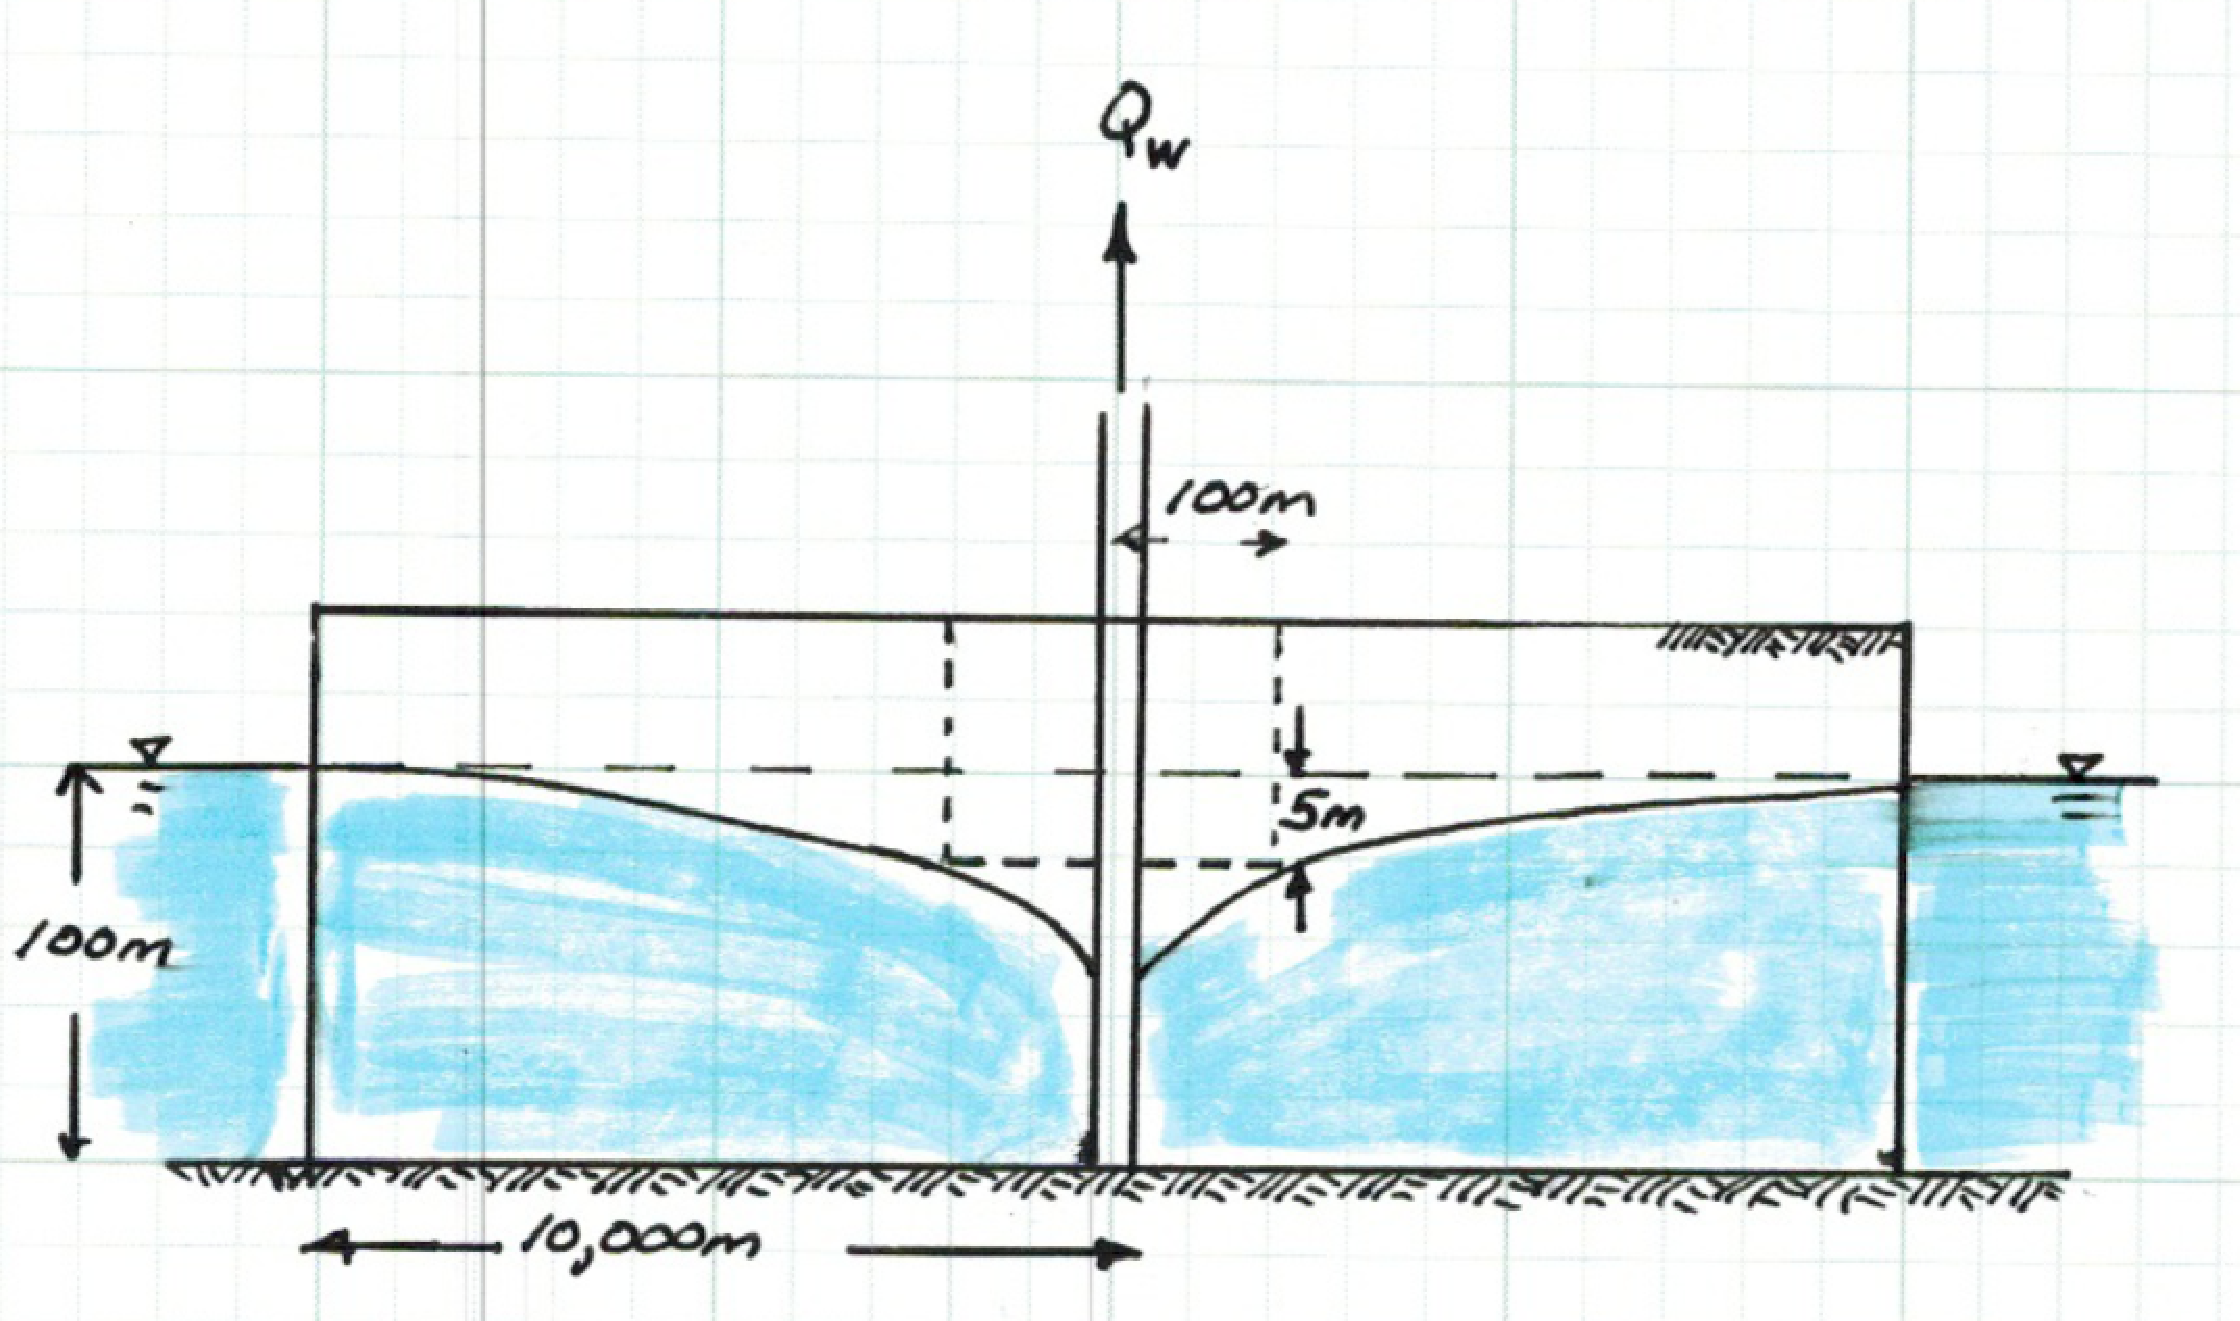
\includegraphics[width=5.5in]{well-in-aquifer.pdf} 
   \caption{Pumping well in circular, unconfined aquifer.}
   \label{fig:well-in-aquifer.pdf}
\end{figure}
\begin{enumerate}
\item What is the head at the center of the island (in the well) before turning on the pump?
\item What is the head 100 meters from the well before turning on the pump?
\item What is the head 10,000 meters from the well before turning on the pump?
\item What is the head 100 meters from the well when the pump is operating at the desired flow rate?
\item What is the head 10,000 meters from the well when the pump is operating at the desired flow rate?
\item Write the equation that relates the pump rate, head, and hydraulic conductivity for a well in an unconfined aquifer.
\item Apply the equation and estimate the required pumping rate to produce the desired head 100 meters from the well.   Show your arithmetic.
\end{enumerate}
%%%%%%%%%%%%%%%%%%%%%%%%%%%%%%%%%%%%%%%%%%%%%%%%%%%%%%%%%%%%%%%%%%%%
\clearpage
\item Figure \ref{fig:aquifer-map.pdf} (next page) is a map of the piezometric surface (head) in the Floridian aquifer.  

\begin{enumerate}
\item What is the head in the aquifer near Altamonte Springs (A1)?
\item What is the head in the aquifer near Sanlando Springs (A2)?
\item What is the head in the aquifer near Lake Mary (A3)?
\item What is the head in the aquifer near Golden Lake (A4)?
\item What is the head in the aquifer near location (A5)?
\item Sketch flowlines near Altamonte Springs (A1).
\item Sketch flowlines near Sanlando Springs (A2).
\item Sketch flowlines near Lake Mary (A3).
\item Sketch flowlines near Golden Lake (A4).
\item Sketch flowlines near location (A5).
\item Based on the flowlines, is Altamonte Springs a recharge or discharge area?  (Explain your reasoning)
\item Based on the flowlines, is Sanlando Springs a recharge or discharge area?  (Explain your reasoning)
\item Based on the flowlines, is Lake Mary a recharge or discharge area?  (Explain your reasoning)
\item Based on the flowlines, is Golden Lake a recharge or discharge area?  (Explain your reasoning)
\item Based on the flowlines, is location (A5) a recharge or discharge area?  (Explain your reasoning)
\begin{figure}[h!] %  figure placement: here, top, bottom, or page
   \centering
   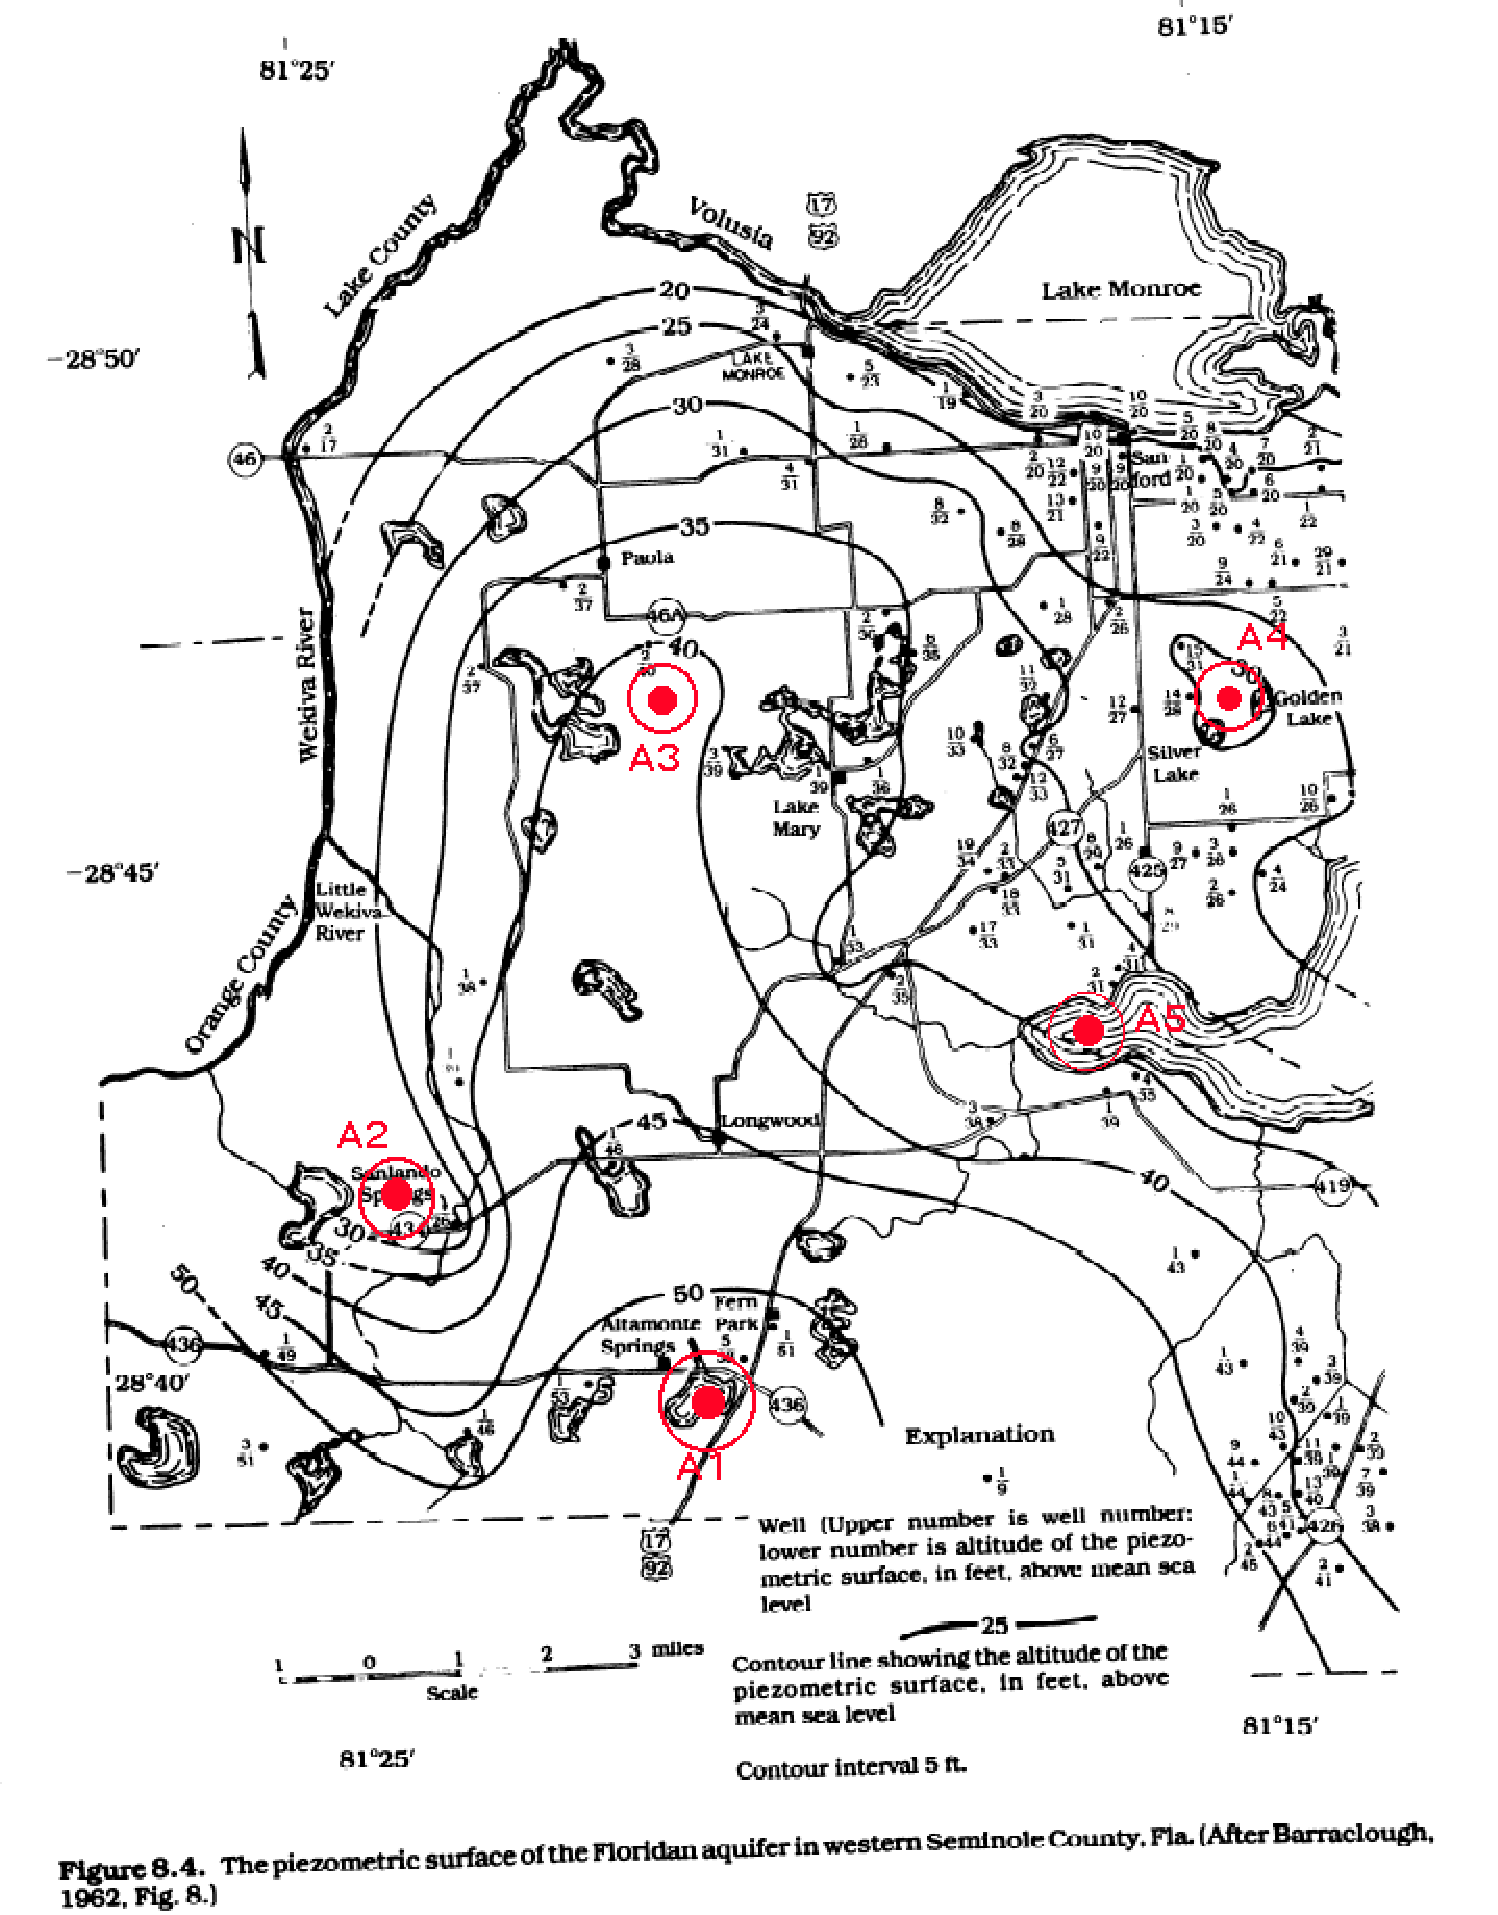
\includegraphics[width=6.2in]{aquifer-map.pdf} 
   \caption{Piezometric surface map of portion of Floridian aquifer.}
   \label{fig:aquifer-map.pdf}
\end{figure}
\clearpage

\end{enumerate}


\end{enumerate}
\end{document}


